\subsection{Declaraciones condicionales}
Las sentencias condicionales en Python permiten controlar el flujo del programa en función del valor de una expresión booleana. Una expresión booleana es una expresión que puede evaluarse como verdadera o falsa.\\

Sentencia if: se considera la más sencilla de las tres y toma decisiones basadas en sí la condición es verdadera o falsa. Si la condición es verdadera, se ejecuta el bloque de código sangrado. Si la condición es falsa, se omite la ejecución del bloque.\\

La sintaxis básica de la condición if es la siguiente:
\begin{figure}[h]
    \centering
    \scalebox{0.35}{
    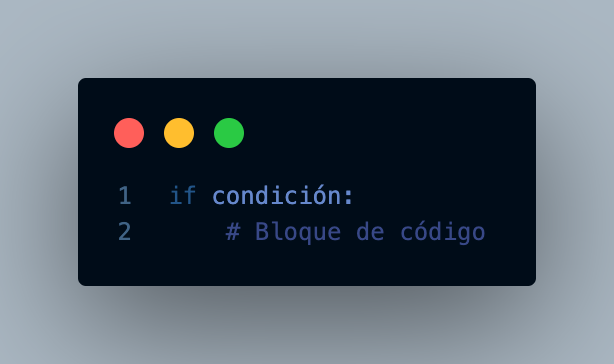
\includegraphics{Imagenes/estructura1.png}
    }
  \end{figure}
\newpage
Por ejemplo, el siguiente código imprime ``El número es mayor que 10'' si el número es mayor que 10:

\begin{figure}[h]
    \centering
    \scalebox{0.35}{
    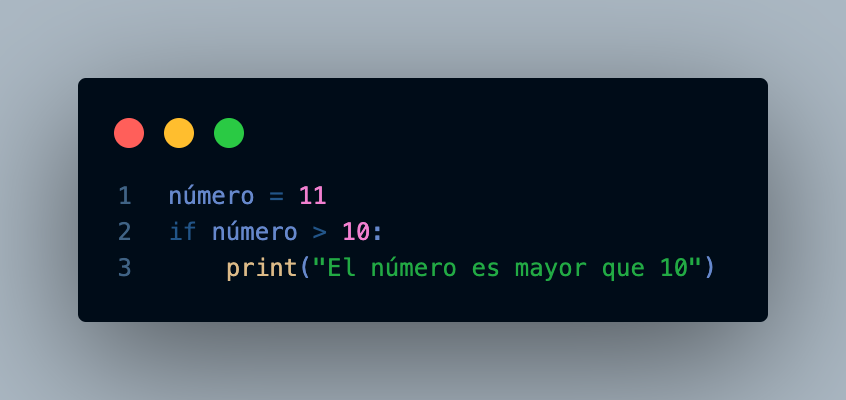
\includegraphics{Imagenes/estructura2.png}
    }
  \end{figure}

En este ejemplo, la condición es que el número sea mayor que 10. El bloque de código contiene una sola instrucción, que es imprimir el mensaje ``El número es mayor que 10''.\\

Sentencia else (opcional): Puedes agregar un bloque de código que se ejecutará si la primera condición es falsa.

La sintaxis básica de la condición else es la siguiente:

\begin{figure}[h]
    \centering
    \scalebox{0.35}{
    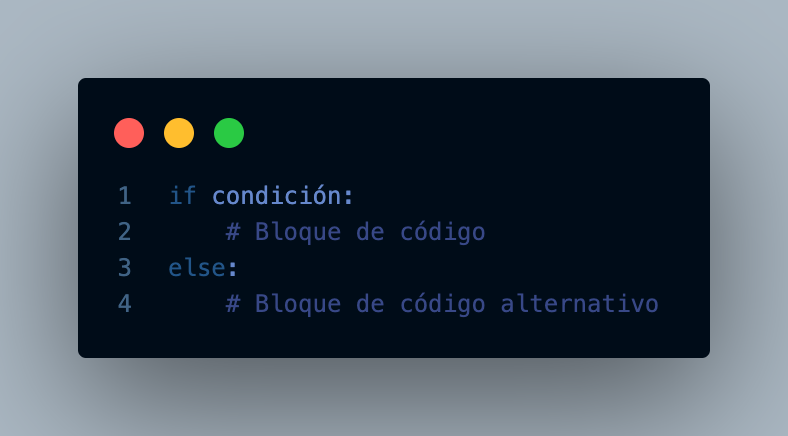
\includegraphics{Imagenes/estructura3.png}
    }
  \end{figure}

Por ejemplo, el siguiente código imprime ``El número es menor que 10'' si el número es menor que 10:

\begin{figure}[h]
    \centering
    \scalebox{0.35}{
    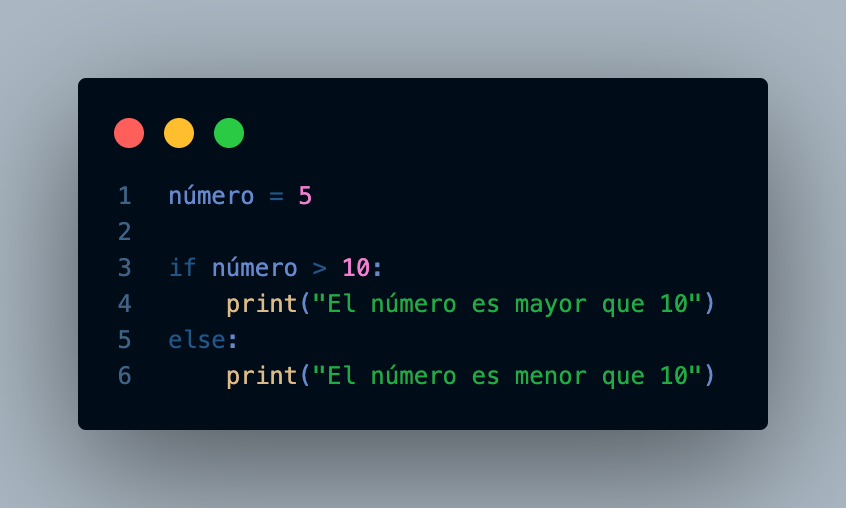
\includegraphics{Imagenes/estructura4.png}
    }
  \end{figure}

En este ejemplo, la condición es que el número sea mayor que 10. El bloque de código principal se ejecuta si la condición es verdadera. Si la condición es falsa, se ejecuta el bloque de código alternativo.\\

Sentencia elif (opcional): Para verificar múltiples condiciones, puedes utilizar elif después de la declaración if. Ten en cuenta que solo se ejecutará el bloque de código correspondiente a la primera condición verdadera.\\

La sintaxis básica de la sentencia elif es la siguiente:
\begin{figure}[h]
    \centering
    \scalebox{0.35}{
    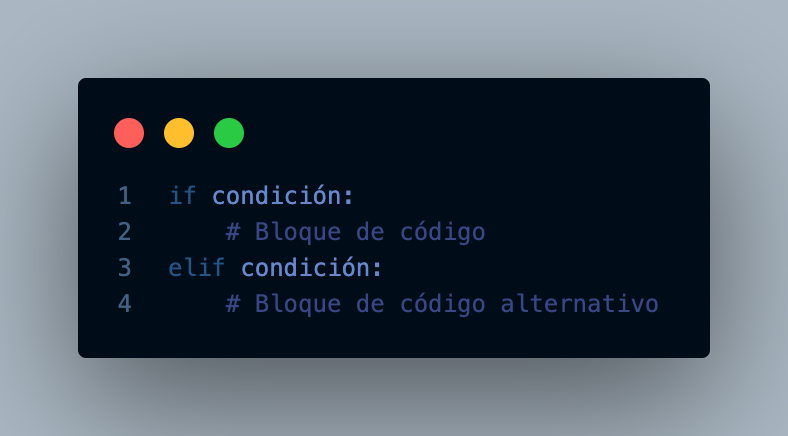
\includegraphics{Imagenes/estructura5.png}
    }
  \end{figure}

Por ejemplo, el siguiente código imprime ``El número es mayor que 10'' si el número es mayor que 10, ``El número es igual a 10'' si el número es igual a 10, y ``El número es menor que 10'' si el número es menor que 10:

\begin{figure}[h]
    \centering
    \scalebox{0.35}{
    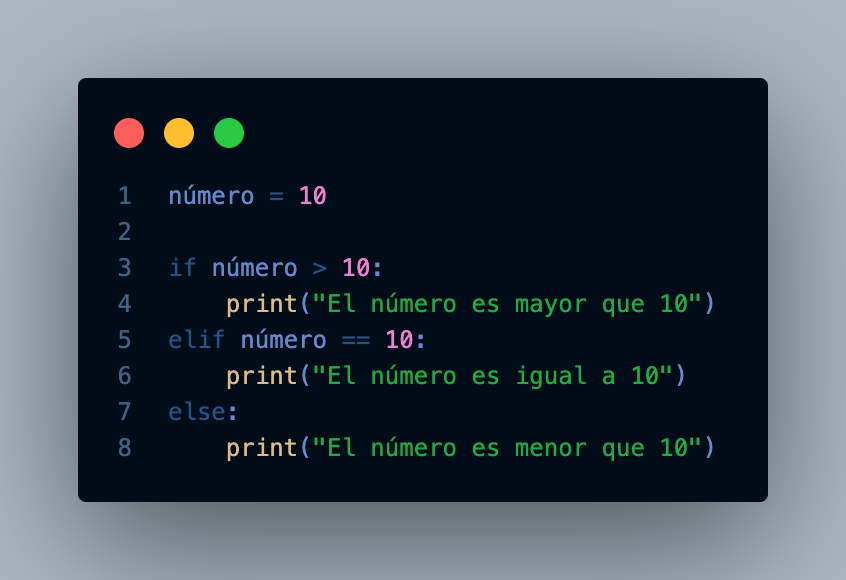
\includegraphics{Imagenes/estructura6.png}
    }
  \end{figure}

En este ejemplo, la condición principal es que el número sea mayor que 10. Si la condición principal es verdadera, se ejecuta el bloque de código principal. Si la condición principal es falsa, se evalúa la primera condición elif. Si la primera condición elif es verdadera, se ejecuta el bloque de código alternativo. Si la primera condición elif es falsa, se evalúa la segunda condición elif, y así sucesivamente. Si ninguna de las condiciones elif es verdadera, se ejecuta el bloque de código else.

\subsection{Bucles y iteraciones}
En el contexto de la programación, los términos loops e iteraciones a menudo se utilizan indistintamente, pero hay una distinción sutil:

\begin{itemize}
    \item Iteración: La iteración se refiere al proceso de repetir una acción o un bloque de código para cada elemento de una secuencia o hasta que se cumpla una condición. La iteración no está limitada a los bucles, ya que puede ocurrir en otros contextos, como al recorrer elementos en una lista o realizar operaciones en un conjunto de datos.
    \item Loop (bucle): Un loop es una estructura de control que permite repetir un bloque de código múltiples veces. Puede ser un ciclo for o ``while'', y generalmente se utiliza cuando se conoce la cantidad de repeticiones necesarias. Un loop puede realizar iteraciones.
\end{itemize}

\subsection{Tipos de bucles en Python}
En Python, existen dos tipos de bucles:
\begin{itemize}
    \item Bucle for: El bucle for se utiliza para iterar sobre una colección de datos. La sintaxis es la siguiente: 
    \begin{figure}[h]
        \centering
        \scalebox{0.35}{
        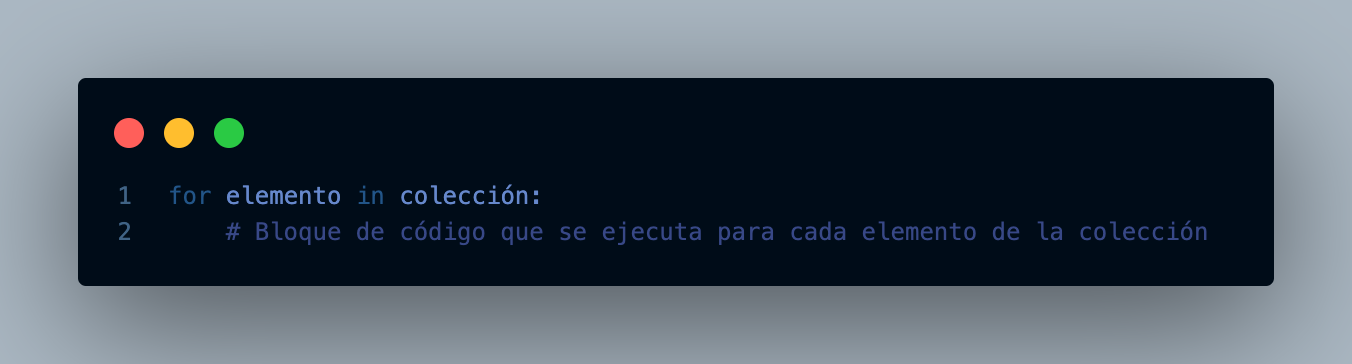
\includegraphics{Imagenes/estructura7.png}
        }
      \end{figure}

      Por ejemplo, el siguiente código imprime los números del 1 al 10:
      \begin{figure}[h]
        \centering
        \scalebox{0.35}{
        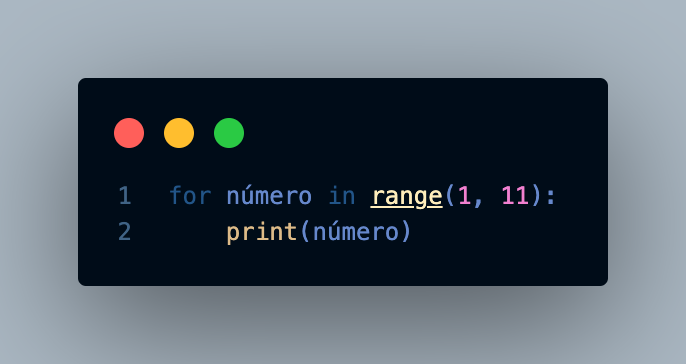
\includegraphics{Imagenes/estructura8.png}
        }
      \end{figure}
\newpage
    \item Bucle while: El bucle while se utiliza para iterar mientras una condición sea verdadera. La sintaxis es la siguiente:
    \begin{figure}[h]
        \centering
        \scalebox{0.35}{
        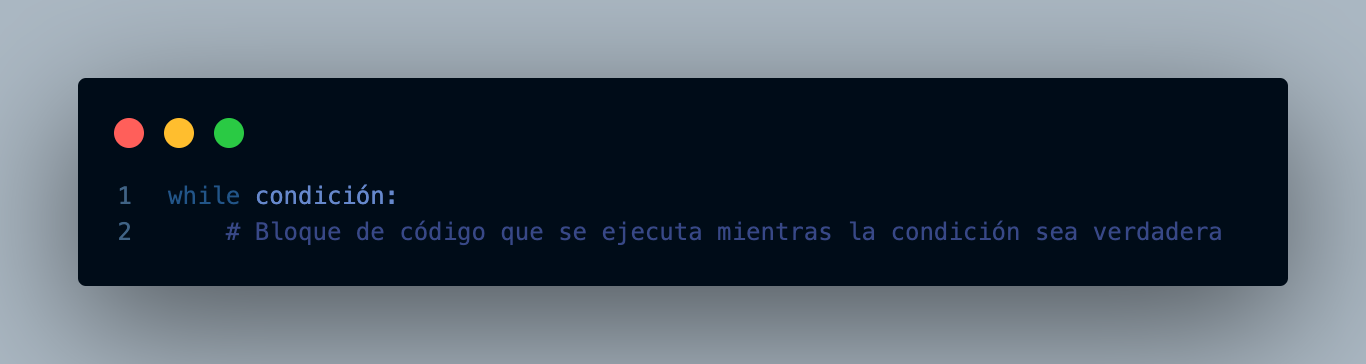
\includegraphics{Imagenes/estructura9.png}
        }
      \end{figure}

      Por ejemplo, el siguiente código imprime los números del 1 al 10:
      \begin{figure}[h]
        \centering
        \scalebox{0.35}{
        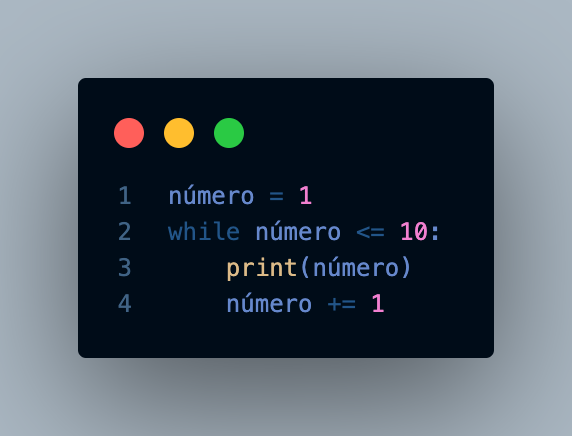
\includegraphics{Imagenes/estructura10.png}
        }
      \end{figure}
\end{itemize}